\section{System design and architecture}
Our system is designed to facilitate a flexible and scalable deployment of applications. The following figure illustrates our system architecture.  

\begin{figure}[h]
\centering
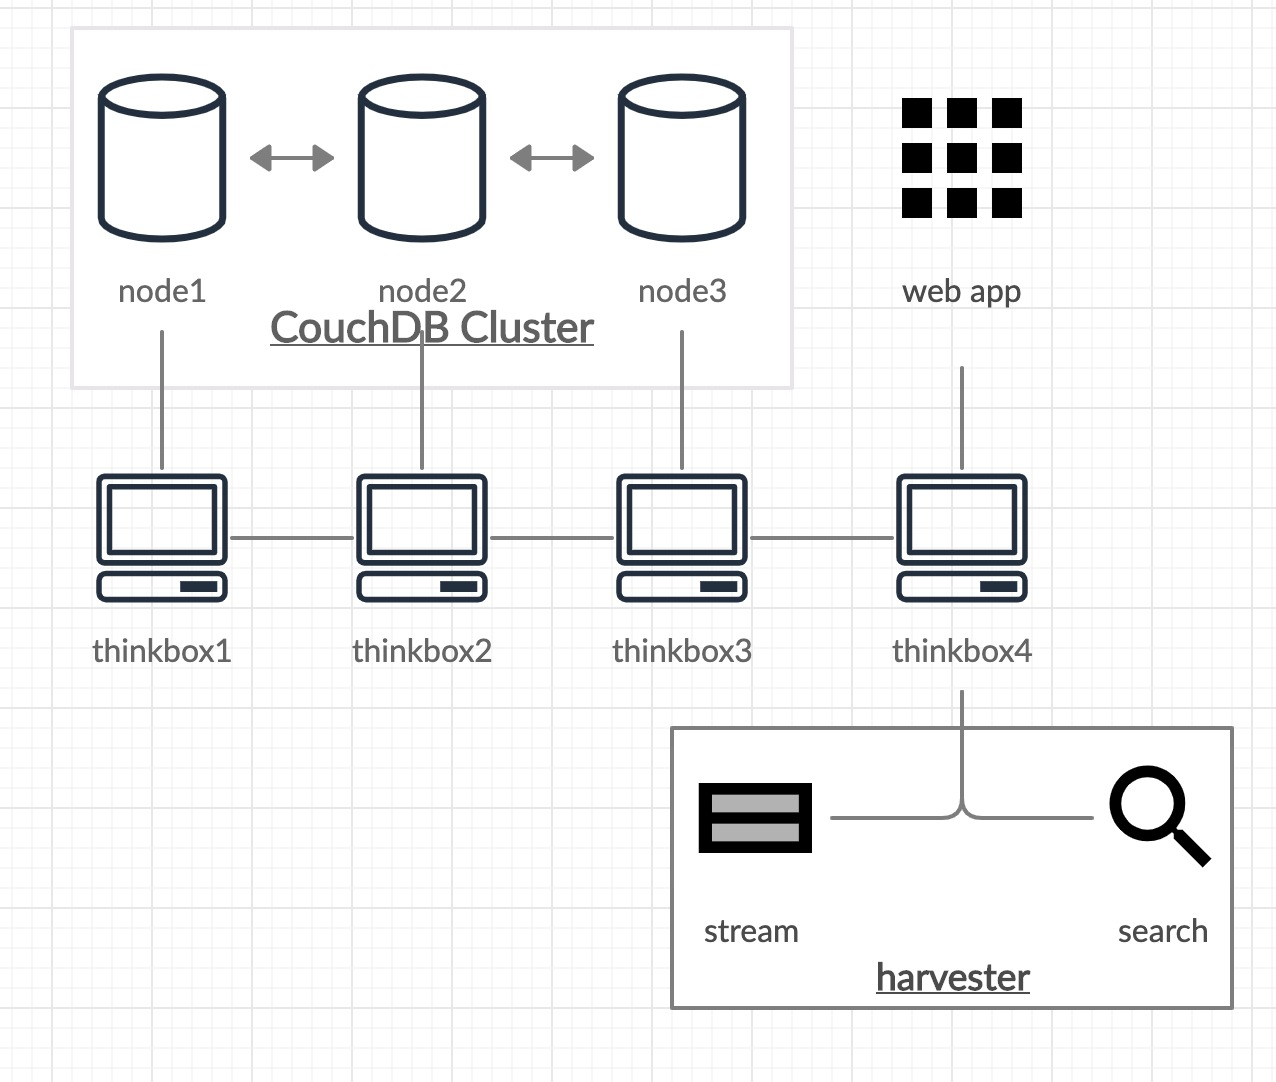
\includegraphics[width=0.5\textwidth]{architecture}
\caption{System architecture}
\end{figure}

All cloud instances are initialized with dynamic IP addresses, which are then exported to a new inventory file. Any application that requires the IP address can parse the inventory file by the instance name. When there is an increased demand on compute instances, we can easily scale up of the system by extending the range in the host-name list (e.g from thinkbox[1:4] to thinkbox[1:50]).  

Our system comprises three main components, including a CouchDB database (to store tweets), a tweet harvester and a geospatial web application (to visualize our scenarios). Any of these components can be run on any node in the Melbourne Research Cloud. In order to attain flexibility of packing and running these components, we foster the use of dockerization. In other words, every application will run inside a Docker container.  

In this project, we experiment with 4 cloud instances and 250 Gb volume for storage. For clarity purposes, these instances will be identified as thinkbox 1, thinkbox 2, thinkbox 3 and thinkbox 4.  

A 3-node CouchDB cluster is set up on Thinkbox 1,2 and 3 due to the high CPU loading which will be further discussed in CouchDB section. This setup allows these 3-nodes to communicate with each other.

Harvester has been divided into two different stages, the first stage is a mass collection of tweets using two different sources, and the second stage is to deploy on one of the cloud instances to run streaming 24*7. A detailed descriptions are covered in Harvester section.

The geospatial web application retrieves tweet data from CouchDB database, which is tagged with geo-location and associated with a scenario that we are interested in, visualizes the statistics and then display the graphs in a web browser. As the database is constantly updated with new tweets, our statistics and graphs will also be reflecting these changes.  

\section{Docker}
Docker containers are used in this project as it allow us to isolate and run multiple components on the cloud instances. Rather than using an instance for each components on the server. This lightweight containers makes it easier to modify and update the program which leads to better resource usage, and higher performance. Dockers are used to deployed all the components.

\subsection{Dockerize CouchDB}

The latest CouchDB docker image is used, it is compatible with Cloudant which is later used in Python to streamline the process of querying and updating the databases. Because Docker does not persist data, the external storage /dev/vdb directory /external is bind mount to mounted to the CouchDB opt/couchdb/data. Therefore, even if the docker has to be terminated, CouchDB can restores the databases. Bind mount is chosen because it is easier to manage and back up, also, it allows us to examine the data directly, although the drawback is that problem in data security arises. 

Following figure shows the CPU process for thinkbox 1,2,3 which are running CouchDB. It varies from as little as 0.6\% to 180\%. However since there is no other application is running on this instances. There is no need to constraints to limit the CouchDB containers to access thinkbox 1,2 and 3 CPU cycles. However if require it can be set by using --cpus="1.5", which at most one and a half of the CPUs is available for the container.

\begin{figure}[h]
\centering
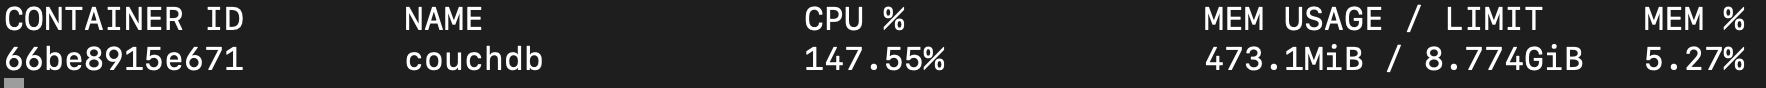
\includegraphics[width=1.0\textwidth]{city_analytics/report/images/CPUthinkbox.png}
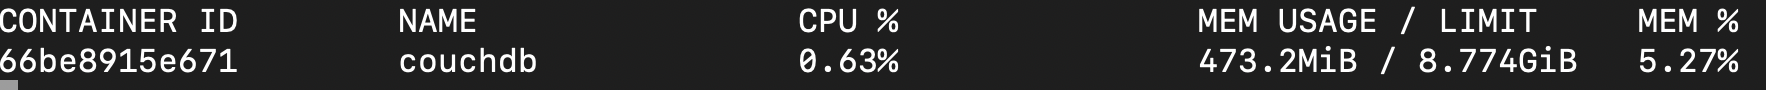
\includegraphics[width=1.0\textwidth]{city_analytics/report/images/couchdb1.png}
\caption{CPUs performance on Thinkbox 1,2 & 3}
\end{figure}

\subsection{Dockerize Harvester}

Harvester application runs majorly on two main Python scripts, main.py and stream.py. These two scripts are dockerize using the Python:3.7-Alpine image. They are binded to /external/harvester on ThinkBox 4. Apart from persisting the data, this was configured to allow data-sharing between containers. The dependencies that are installed are Tweepy, Couchdb, Cloudant, Textblob and Schedule. Alpine image is used as it is smaller and may speed up the builds if the dependencies does not require standard PyPI wheels . In this case, the size of the image is 91.7Mb. Since the scripts are schedule to run on certain time, especially during off-peak hours, the timezone is changed using ENV TZ Australia/Melbourne in dockerfile. Figure ~\ref{fig:thinkbox4}, shows that the main.py has the highest CPU \%, but not significantly in a way that detriment thinkbox4. The container named views runs a small python script that periodically updates databases views and filters a database called 'Tweet-Covid-Symptoms'.

\begin{figure}[h]
\centering
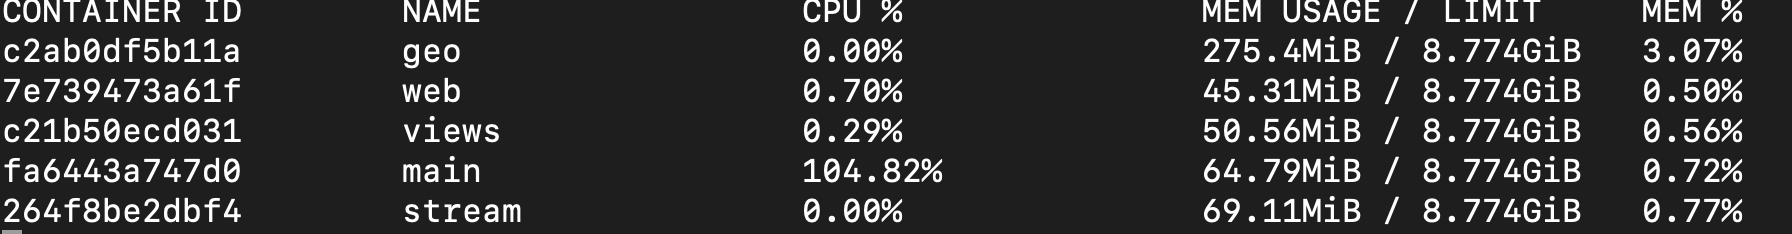
\includegraphics[width=1.0\textwidth]{city_analytics/report/images/thinkboxCPU.png}

\caption{CPUs performance on Thinkbox 4}
\label{fig:thinkbox4}
\end{figure}


\subsection{Dockerize Web App}

The web-app runs on two Python scripts and are dockerized to the containers labelled as geo and web. Geo task requires pandas, geopandas, IPython, cloudant, folium and matplotlib. These dependenecies do not work well with Alpine, installing these dependencies will takes a longer time to build. Python:3.8-Slim is used instead as it supports the manylinux1 wheels and also saves considerable time and space comparatively. Container "Web" only requires Flask and Cloudant which again built on 3.7 Alpine. These containers are bind mounted to the /external/front directory to allow Python-Flask acquires the html output from Geo. 
